\subsection{Einlesen der Konfigurationsdateien}
\paragraph{Klassenstruktur}
Im Backend (falls man es so nennen kann) wird die Klassenstruktur der \acs{gui} nachgebildet. Es gibt eine Page-, Measurement- und Sensorklasse. Ein Measurement kann mehrere Sensoren enthalten, da manche Measurements zur Berechnung  (z.B. der Wärmerückgewinnungsgrad) mehrere Messwerte benötigen. Die Pages speichern die jeweiligen Measurements, die auf dieser Seite angezeigt werden sollen. Die Pages existieren, damit der ausgelesene Parameter an der richtigen Stelle auf der \acs{gui} verändert werden kann. Es gibt nämlich gleich viele Pages Objekte wie GuiPages Objekte und gleich viele Measurement Objekte wie MeasurementFrame Objekte. (siehe Abb.~\ref{fig:uml_backend}).
\begin{figure}[ht]
	\centering
	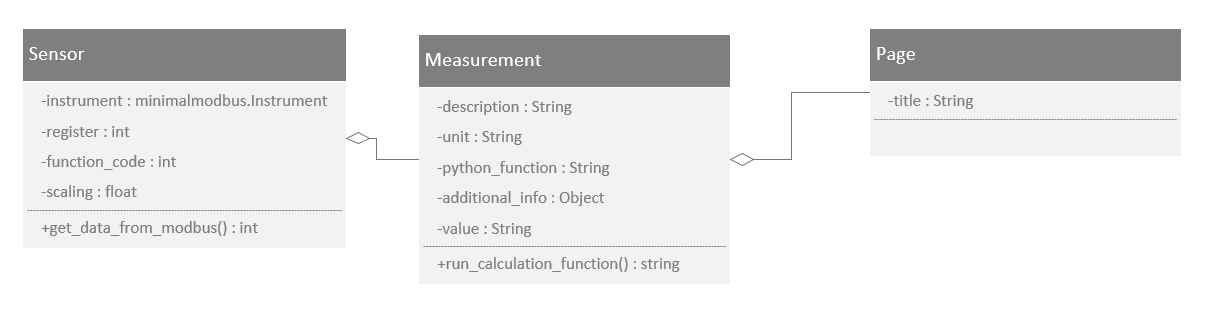
\includegraphics[width=1.0\linewidth]{Bilder/UML_Backend}
	\caption{UML Diagramm Backend}
	\label{fig:uml_backend}
\end{figure}

Die Page-, Measurement- und Sensorobjekte werden beim Einlesen der Konfigurationsdateien aufgrund des \enquote{pages} JSON Objekts erstellt und in Listen gespeichert. \newline
Zum Einlesen werden drei Funktionen implementiert:
\begin{itemize}
	\item \textbf{\enquote{load\_config}:} Diese Funktion lädt die gesamte Hauptkonfigurationsdatei ein. Es werden die angeschlossenen Geräte ermittelt und die Page-, Measurement- und Sensorobjekte erstellt. Dafür kommen die beiden folgenden Hilfsfunktionen zum Einsatz.
	\item \textbf{\enquote{get\_sensor\_unit}:} Liest die Sensor-Konfigurationsdateien ein. Dadurch können den Messwerten die richtigen Maßeinheiten zugewiesen werden.
	\item \textbf{\enquote{get\_sensor\_data}:} Liest aus der Geräte-Konfigurationsdatei am angegebenen Port die Parameter aus und liefert diese Parameter als JSON Objekt zurück. Sie liest das Register, den Function Code und die Skalierung aus. Die Skalierung wird anhand der Maßeinheit aus der Sensor-Konfigurationsdatei ausgewählt.
\end{itemize}

\paragraph{Einlesen und erstellen der Objektstruktur}
Einlesen kann man ein JSON Attribut mit folgender Syntax. Im folgenden Beispiel wird aus dem Objekt namens page das Attribut title gesucht und zurückgeliefert.
\begin{pythoncode}
title = page["title"]
\end{pythoncode}

Im folgenden Code werden die Measurements erstellt, indem die anzuzeigenden Messwerte aus dem Sources Array iteriert werden. Anhand der Informationen im Sources Array werden dann die entsprechenden Geräte im Devices Array herausgesucht. Es werden weitere Parameter aus der Hauptkonfiguration ausgelesen, die zu dem entsprechenden Messwert gehören (z.B. die Beschreibung oder die Einheit). Anschließend werden die Sensorobjekte erstellt (Verweis auf nächsten Codeblock) und einer Liste beigefügt, da manche Measurements mehrere Messwerte benötigen. Diese Liste, sowie die vorher ausgelesenen Parameter werden beim Erstellen der Measurement Objekte dem Konstruktor übergeben und darin in Instanzvariablen gespeichert.
\begin{pythoncode}
page_measurements = []
for measurements in page["sources"]:
	page_sensors = []
	[Auslesen weiterer Parameter der Hauptkonfigurationsdatei (description, unit, python_function,additional_info)]
	[Erstellen der Sensorobjekte (Verweis auf nächsten Codeblock)]
	page_measurements.append(Measurement(description=description, unit=unit, sensors=page_sensors, python_function=python_function, additional_info=additional_info))
\end{pythoncode}

Im folgenden Code wird für jeden Port (an jedem Port ist ein Sensor angeschlossen) eines Geräts ein Sensorobjekt erstellt. Alle Sensorobjekte werden der \enquote{page\_sensors} Liste beigefügt. Dafür gibt es im Sources Array die einzelnen Ports. Das sind Wertepaare, die aus Gerät und Sensor bestehen (vgl. Kapitel damio). Mit diesen beiden Werten kann dann das entsprechende Gerät im Devices Array gefunden werden und darin der entsprechende Port im Sensors Array. Mit der \enquote{get\_sensor\_unit} wird die Einheit erhalten und mit \enquote{get\_sensor\_data} weitere Sensordaten. Diese werden beim Erstellen des Sensorobjekts dem Konstruktor übergeben.
\begin{pythoncode}
port_counter = 0
for port in port_arr:
	device_id = list(port.keys())[port_counter] # example: QBM1
	port_id = port[device_id]  # example: AI1
	port_counter += 1
	
	for device in config_full_data[0]["devices"]:
		if device["id"] == device_id:
			[Aufruf der get_sensor_unit Funktion]
			%[Auslesen der Geräteparameter in der Hauptkonfigurationsdatei (baud_rate, mbaddress etc.)]
			[Aufruf der get_sensor_data Funktion]
			page_sensors.append(Sensor(baud_rate=device["baud_rate"], [...], register=register, zero_based=device["zero_based"]))	
\end{pythoncode}

Die Measurements sind nach dem Erstellen alle in einer Liste gespeichert. Zum Schluss werden Pageobjekte erstellt. Die Measurements Liste wird so aufgeteilt, dass maximal 5 Measurements auf einer Seite sind. Anhand von diesen Page- und Measurement Objekten wird beim Erstellen der \acs{gui} die Anzahl an Seiten übernommen und der Seitentitel und die Beschreibungen der Messwerte gesetzt (siehe Kapitel GUI beschreibung). 
\begin{pythoncode}
counter = 0
last_slice = 0
for measurement in page_measurements:
	counter += 1
	if ((counter \% 5) == 0) or (counter == len(page_measurements)):
		all_pages.append(Page(title=title, measurements=page_measurements[last_slice:counter]))
		last_slice = counter
\end{pythoncode}

%\pythonfile[firstline=125, lastline=197]{Code/modbus.py}

Im Konstruktor der Page- Measurement- und Sensorobjekte werden die ausgelesenen Variablen in Instanzvariablen gespeichert.